\documentclass[
	12pt,				% tamanho da fonte
	openright,			% capítulos começam em pág ímpar (insere página vazia caso preciso)
	twoside,			% para impressão em recto e verso. Oposto a oneside
	a4paper,			% tamanho do papel. 
	% -- opções da classe abntex2 --
	%chapter=TITLE,		% títulos de capítulos convertidos em letras maiúsculas
	%section=TITLE,		% títulos de seções convertidos em letras maiúsculas
	%subsection=TITLE,	% títulos de subseções convertidos em letras maiúsculas
	%subsubsection=TITLE,% títulos de subsubseções convertidos em letras maiúsculas
	% -- opções do pacote babel --
	english,			% idioma adicional para hifenização
	french,				% idioma adicional para hifenização
	spanish,			% idioma adicional para hifenização
	brazil				% o último idioma é o principal do documento
	]{abntex2}

% ---
% Pacotes básicos 
% ---
\usepackage{lmodern}			% Usa a fonte Latin Modern			
\usepackage[T1]{fontenc}		% Selecao de codigos de fonte.
\usepackage[utf8]{inputenc}		% Codificacao do documento (conversão automática dos acentos)
\usepackage{indentfirst}		% Indenta o primeiro parágrafo de cada seção.
\usepackage{color}				% Controle das cores
\usepackage{graphicx}			% Inclusão de gráficos
\usepackage{microtype} 			% para melhorias de justificação
% ---
		

% ---
% Pacotes de citações
% ---
\usepackage[brazilian,hyperpageref]{backref}	 % Paginas com as citações na bibl
\usepackage[alf]{abntex2cite}	% Citações padrão ABNT

% --- 
% CONFIGURAÇÕES DE PACOTES
% --- 

% ---
% Configurações do pacote backref
% Usado sem a opção hyperpageref de backref
\renewcommand{\backrefpagesname}{Citado na(s) página(s):~}
% Texto padrão antes do número das páginas
\renewcommand{\backref}{}
% Define os textos da citação
\renewcommand*{\backrefalt}[4]{
	\ifcase #1 %
		Nenhuma citação no texto.%
	\or
		Citado na página #2.%
	\else
		Citado #1 vezes nas páginas #2.%
	\fi}%


% ---
% Informações de dados para CAPA e FOLHA DE ROSTO
% ---
\titulo{A linguagem C e as vicissitudes da compilação.}
\autor{Gabriel Gian}
\local{Guaxupé, Minas Gerais}
\data{2021}
\instituicao{
Centro Universitário da Fundação Educacional Guaxupé\\ -- UNIFEG}
\tipotrabalho{Trabalho}



% ---
% Configurações de aparência do PDF final

% alterando o aspecto da cor azul
\definecolor{blue}{RGB}{41,5,195}

% informações do PDF
\makeatletter
\hypersetup{
     	%pagebackref=true,
		pdftitle={\@title}, 
		pdfauthor={\@author},
    	pdfsubject={\imprimirpreambulo},
	    pdfcreator={LaTeX with abnTeX2},
		pdfkeywords={abnt}{latex}{abntex}{abntex2}{trabalho acadêmico}, 
		colorlinks=true,       		% false: boxed links; true: colored links
    	linkcolor=blue,          	% color of internal links
    	citecolor=blue,        		% color of links to bibliography
    	filecolor=magenta,      		% color of file links
		urlcolor=blue,
		bookmarksdepth=4
}
\makeatother
% --- 

% ---
% Posiciona figuras e tabelas no topo da página quando adicionadas sozinhas
% em um página em branco. Ver https://github.com/abntex/abntex2/issues/170
\makeatletter
\setlength{\@fptop}{5pt} % Set distance from top of page to first float
\makeatother
% ---

% ---
% Possibilita criação de Quadros e Lista de quadros.
% Ver https://github.com/abntex/abntex2/issues/176
%
\newcommand{\quadroname}{Quadro}
\newcommand{\listofquadrosname}{Lista de quadros}

\newfloat[chapter]{quadro}{loq}{\quadroname}
\newlistof{listofquadros}{loq}{\listofquadrosname}
\newlistentry{quadro}{loq}{0}

% configurações para atender às regras da ABNT
\setfloatadjustment{quadro}{\centering}
\counterwithout{quadro}{chapter}
\renewcommand{\cftquadroname}{\quadroname\space} 
\renewcommand*{\cftquadroaftersnum}{\hfill--\hfill}

\setfloatlocations{quadro}{hbtp} % Ver https://github.com/abntex/abntex2/issues/176
% ---

% --- 
% Espaçamentos entre linhas e parágrafos 
% --- 

% O tamanho do parágrafo é dado por:
\setlength{\parindent}{1.3cm}

% Controle do espaçamento entre um parágrafo e outro:
\setlength{\parskip}{0.2cm}  % tente também \onelineskip

% ---
% compila o indice
% ---
\makeindex
% ---

% ----
% Início do documento
% ----
\begin{document}

% Seleciona o idioma do documento (conforme pacotes do babel)
\selectlanguage{brazil}

% Retira espaço extra obsoleto entre as frases.
\frenchspacing 

% ----------------------------------------------------------
% ELEMENTOS PRÉ-TEXTUAIS
% ----------------------------------------------------------
% \pretextual

% ---
% Capa
% ---
\imprimircapa
% ---

% ---
% Folha de rosto
% (o * indica que haverá a ficha bibliográfica)
% ---
\imprimirfolhaderosto*

\begin{fichacatalografica}
	\sffamily
	\vspace*{\fill}					% Posição vertical
	\begin{center}					% Minipage Centralizado
	\fbox{\begin{minipage}[c][8cm]{13.5cm}		% Largura
	\small
	\imprimirautor
	%Sobrenome, Nome do autor
	
	\hspace{0.5cm} \imprimirtitulo  / \imprimirautor. --
	\imprimirlocal, \imprimirdata-
	
	\hspace{0.5cm} \thelastpage p. : il. (algumas color.) ; 30 cm.\\
	
	\hspace{0.5cm} \imprimirorientadorRotulo~\imprimirorientador\\
	
	\hspace{0.5cm}
	\parbox[t]{\textwidth}{\imprimirtipotrabalho~--~\imprimirinstituicao,
	\imprimirdata.}\\
	
	\hspace{0.5cm}
		1. Linguagens de programação
		2. Linguagem de programação C
		I. UNIFEG
	\end{minipage}}
	\end{center}
\end{fichacatalografica}

\chapter{Introdução}

No fim dos anos 70, a AT\&T licenciou o sistema operacional Unix desenvolvido nos seus Bell Labs, por Ken Thompson e Dennis Ritchie, no começo daquela mesma década. O desenvolvimento deste sistema, sendo o mesmo praticamente um filho de uma ideia abortada --- o sistema de tempo compartilhado Multics --- que se mostrou demasiadamente complexo e impraticável em termos de tamanho e tecnologia disponível. O sistema Unix, inicialmente, estava sendo implementado em linguagem assembly para o computador portátil PDP-11, mas o gargalo de complexidade apresentado por este método acabou criando a necessidade de engendrar uma tecnologia que se mostraria ainda mais importante que o próprio Unix. \par 
Era o nascimento da linguagem C.
\chapter{Breve história da linguagem C}

Desenvolvida por Dennis Ritchie, durante o ciclo de desenvolvimento do Version 4 Unix, a linguagem C nasceu como uma sucessora direta da linguagem \textit{B}, de seu parceiro de desenvolvimento (e Prêmio Turing) Ken Thompson, linguagem que por si própria era uma evolução da sua linguagem anterior, \textit{Bon}. A linguagem buscava ser uma alternativa de alto nível, apresentando um bom grau de abstração em relação ao código de máquina, embora que ainda mantenha um excelente grau de capacidades de manipulação baixo nível --- o que torna-a perfeita para o desenvolvimento de sistemas operacionais. \par
A linguagem C, desde então, foi adotada como uma das linguagens mais amplamente utilizadas, tanto na academia como na indústria, sendo a energia motriz de softwares que vão desde drivers, sistemas embarcados e programas para o processamento veloz de dados requeridos pela matemática computacional, a aplicativos de produtividade, motores de videogames diversos e softwares de controle de aparelhos conectados à dita \textit{Internet das Coisas}. \par


\chapter{''Computação'' começa com C}

A linguagem C é notória por ser praticamente uma abstração mais legível e com mais implementações de estruturas de dados que uma primitiva linguagem de montagem como a assembly do PDP-11 utilizado por Thompson e Ritchie para a implementação do Unix. A linguagem, sendo inspirada em ALGOL e FORTRAN, apresenta a famosa e influente sintaxe imperativa e procedural com blocos separados por chaves (\{\}), representando escopos de código como corpos de funções (métodos) e estruturas de controle como blocos \textit{if --- else} e \textit{switch} condicionais. \par

\begin{figure}[h]
\centering
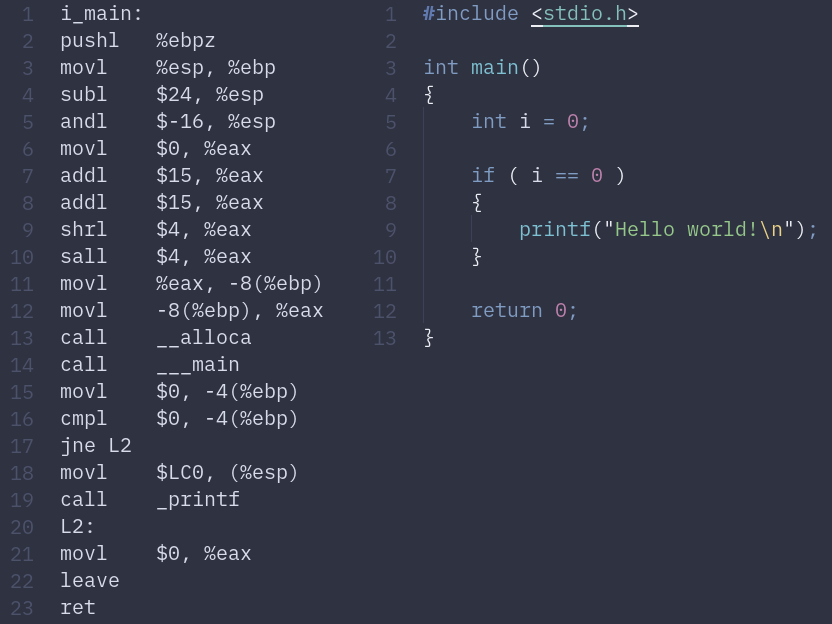
\includegraphics[width=0.6\linewidth]{exemplo.png}
\caption{Exemplo de código assembly e o seu equivalente em C. Nota-se a legibilidade impressionante da relação entre as duas --- o grande chamativo da linguagem C.}
\label{fig:exemplo.png}
\end{figure}

Como se pode ver pelo exemplo acima, a linguagem C é capaz de ser compilada de maneira otimizada (devido aos diversos e maduros compiladores desenvolvidos para implementá-la, como o original \textit{cc} criado por Thompson e Ritchie para o Unix, o moderno \textit{GCC}, do projeto GNU de Richard Stallman, ou a infraestrutura de compilação ainda mais moderna \textit{LLVM}, apoiada pela Apple como concorrente ao GCC, na famosa troca da arquitetura de seus dispositivos de IBM para Intel) para código objeto nativo de praticamente todas as arquiteturas, devido à sua ampla aceitação. \par


\chapter{Futuro}

O futuro da linguagem C pode ser discutido por via de diversos pontos de vista. Há pesquisadores e cientistas da computação que acreditam tratar-se de uma tecnologia atemporal, o que de fato pode ser verdade, uma vez que a linguagem C funciona como uma quase perfeita e simples abstração do código de máquina para níveis de código mais legíveis ao ser humano. A ergonomia da linguagem C é indiscutivelmente bela e produtiva. A linguagem C foi capaz de até mesmo chegar ao espaço, uma vez que diversos programas de controle de robôs e satélites são implementados em C devido à sua velocidade graças à otimização eficiente pelos compiladores modernos de C. Até mesmo outras linguagens são implementadas em C, como Ruby e Python, e há ainda implementações de linguagens declarativas mais antigas que o próprio C como a linguagem Lisp, com a implementação CLISP por Bruno Haible e Michael Stoll. \par 

Há, todavia, o ponto de vista contrário, que enxerga a linguagem C como uma tecnologia do passado --- suas "dificuldades" sendo enxergadas como empecilhos ineficientes para o programador moderno, acostumado ao gerenciamento de memória automático e às facilidades de depuração e distribuição das linguagens modernas. Com o tempo, o surgimento de linguagens com a pretensão de substituir a linguagem C tem engendrado interessantes candidatos modernos ao posto, tendo a linguagem Rust, ao que tudo indica, a melhor chance de executar tal feito, uma vez que já tem sido usada para implementar e até reescrever (o que não é recomendado pela própria comunidade Rust, em nome do enorme respeito pela linguagem C) aplicações baixo nível originalmente implementadas em C. Sinal maior de que a linguagem Rust está em ascensão neste campo não há senão a notícia de que o kernel Linux tem implementado cada vez mais módulos, drivers e APIs em Rust, seu próprio criador, Linus Torvalds, tendo dito em 2020 que apoia a implementação de partes do código em Rust, embora de maneira parcimoniosa. \par  

\chapter{Conclusão}

A linguagem C tem percorrido um longo caminho desde a sua concepção nas Bell Labs. Ela possibilitou um salto tecnológico enorme entre os grandes mainframes e microcomputadores monótonos de outrora, o desenvolvimento de sistemas operacionais cada vez mais potentes e úteis, até mesmo de outras linguagens que trouxeram a computação dos grandes centros de tecnologia militar americana às palmas de nossas mãos. É de suma importância reconhecer o valor inestimável que a linguagem possui, mas é também igualmente importante reconhecer que ela deve ser melhorada, não só nominalmente, mas também conceitualmente, mas centenas de linguagens que dela foram engendradas, e que continuarão a carregar seu legado na eterna jornada de desenvolvimento tecnológico da nossa raça. \par

\chapter{Referências bibliográficas}

RITCHIE, Dennis. \textit{The development of the C language}. Março 1993. Disponível em: https://dl.acm.org/doi/10.1145/155360.155580. Acesso em 20 março 2021.

JOHNSON, Stephen; RITCHIE, Dennis. (1978). \textit{Portability of C Programs and the UNIX System}. Bell System Tech. J. 57 (6): 2021–2048. DOI: 10.1002/j.1538-7305.1978.tb02141.x. Disponível em: https://citeseerx.ist.psu.edu/viewdoc/summary?doi=10.1.1.138.35. Acesso em 23 março 2021.

\textit{A Brief History of GCC}. Disponível em: https://gcc.gnu.org/wiki/History. Acesso em 23 março 2021.

\textit{The LLVM Compiler Infrastruture}. Disponível em: https://llvm.org. Acesso em 23 março 2021.

LARABEL, Michael. \textit{Linus Torvalds' Initial Comment On Rust Code Prospects Within The Linux Kernel}. Disponível em: https://www.phoronix.com/scan.php?page=news_item&px=Linux-Kernel-Rust-PPC64LE.

\end{document}
